\chapter{Examining the Generalisability of Automatic Most Likely Catalogue Matching}\label{ch:SNNGeneralisation}

As outlined in Chapter \ref{ch:ID}, an automatic approach to most likely catalogue matching was developed through the use of Siamese Neural Networks (SNNs). This approach, when tested using the NDD AU SMRU dataset developed in Chapter \ref{ch:NDD}, yields high top-1, top-5, and top-10 accuracies. However, it is not yet clear if these results are to be expected regardless of the photo-id catalogue utilised, or if there is an underlying property inherent to the NDD AU SMRU dataset that makes it particularly susceptible to an SNN-based approach. In this Chapter, automatic most likely matching is performed on a second, previously unseen, photo-id catalogue, allowing for an evaluation of the approach's generalisability.

\section{The SDRP Dataset}\label{ch:SNNGeneralisation,sec:SDRPDataset}

To evaluate the SNN approach's generalisability, a subset of photo-id catalogue data was obtained from the Chicago Zoological Society's Sarasota Dolphin Research Program (SDRP). The subset consisted of 250 images of 23 individual common bottlenose dolphins captured in the waters around Naples, FL, USA \cite{tyson_moore_final_2020}. Unlike the datasets collected from fieldwork in Northumberland, UK, the SDRP dataset was provided in a pre-processed form as the dataset had been previously utilised to compare photo-id methodologies \cite{tyson_moore_rise_2022}. Images provided were cropped to remove a large amount of background noise and centre the dorsal fin, examples of which can be seen in Figure \ref{fig:sdrp-example}. 

\begin{figure}
	\begin{center}
		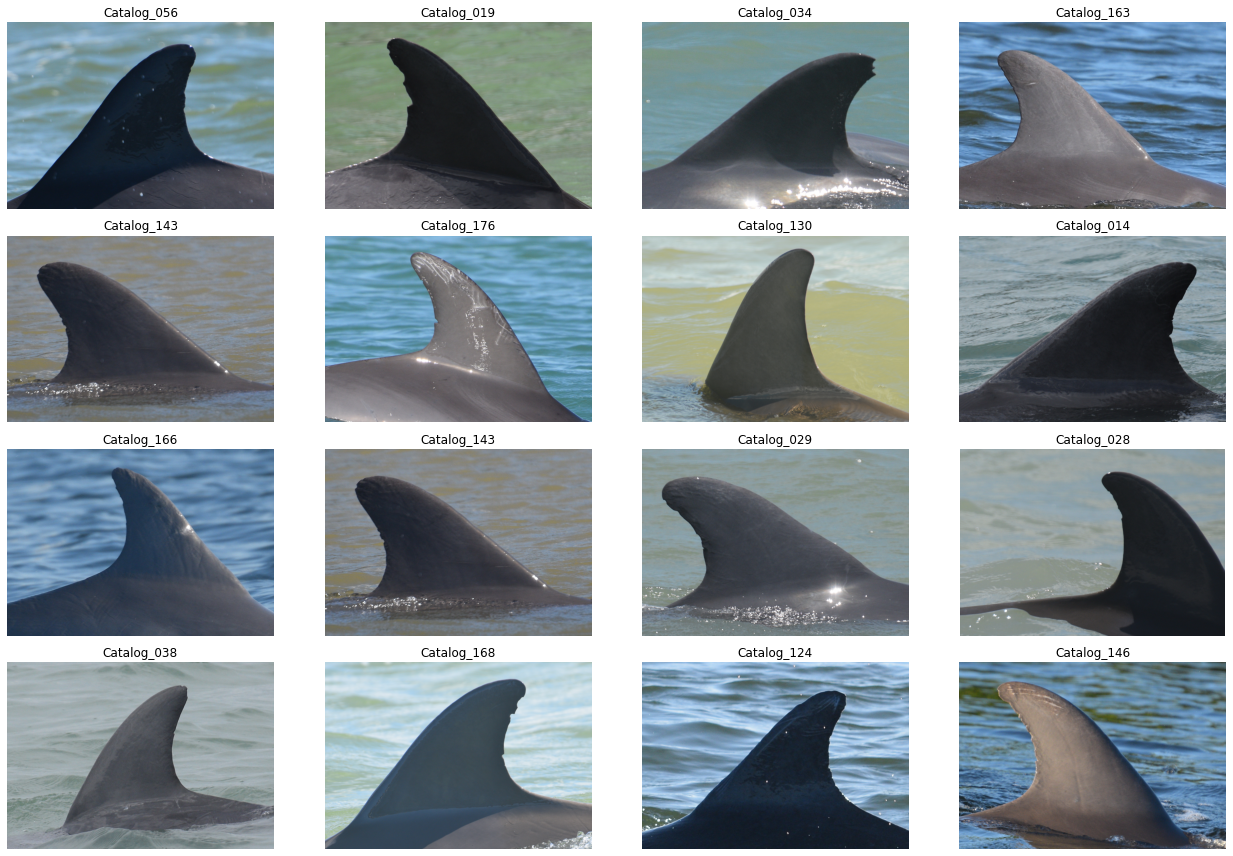
\includegraphics[scale=0.3]{Chapter6/figs/SDRP_egs_tiled.png}
	\end{center}
	\caption{Example images from the SDRP dataset with filenames displayed.}
	\label{fig:sdrp-example}
\end{figure}

The SDRP data was provided pre-split with 200 images, each of a unique individual, acting as the existing photo-id catalogue and the remaining 50 serving as images captured during a given day's fieldwork. Each image in the encounter set also contained a single individual however some individuals were captured multiple times. As such, there was a 23 individual overlap between the catalogue and encounter sets. 

To generate a train-test split capable of training an SNN, the catalogue set was reduced down to contain only the 23 individuals contained within the encounter set. Once filtered, both sets of images were ran through the Mask R-CNN dorsal fin detector and post processed using the methodology outlined in Section \ref{ch:cetDet,sec:postProcessing}. No images in this data had been seen by the detector, either during training or previous evaluation. Once generated, a \texttt{noise} class was manually created which contained all erroneously detected mask components. As the detector failed to accurately detect individual \texttt{19}, all components were marked as \texttt{noise}, resulting in a 23 class dataset. In cases where the detector had mistakenly detected the same fin twice, provided the two masks were not identical then both masks were kept - analogous to offline data augmentation. An example of this can be seen in Figure \ref{fig:sdrp-double-mask-eg}.

\begin{figure}
	\begin{center}
		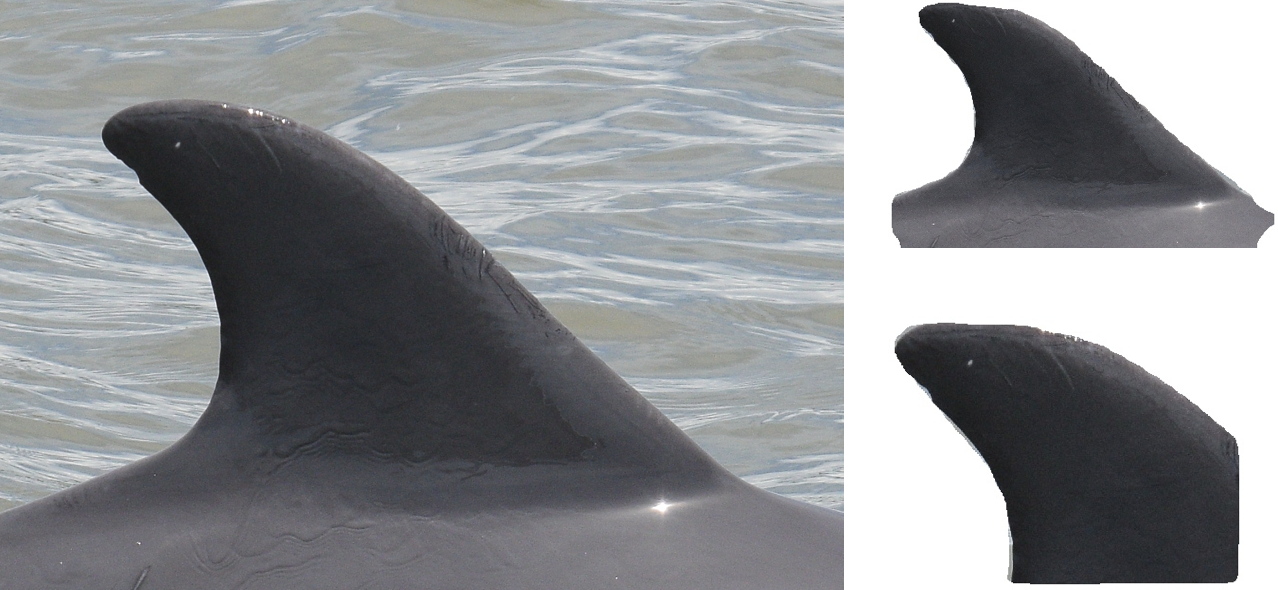
\includegraphics[scale=0.5]{Chapter6/figs/SDRP-double-mask-eg-indv-13.png}
	\end{center}
	\caption{Left: Image of individual \texttt{13} from the original SDRP catalogue set. Right: Example masks generated for the Left image. Both masks are kept for use in training as they were deemed to be sufficiently different.}
	\label{fig:sdrp-double-mask-eg}
\end{figure}

After detection and processing the resultant SDRP dataset contained a total of 123 images, significantly smaller than the NDD AU SMRU dataset which was used to evaluate the SNN-based approach previously. Retaining the split provided by the SDRP whereby the train set was generated from the catalogue and the test set from the encounter leads to a 35-65 train-test split, an inversion of what would be expected when training machine learning models. The class distribution for the SDRP dataset can be seen in Figure \ref{fig:sdrp-dist}. As like with the NDD AU SMRU dataset, the \texttt{noise} class is once again dominant. A colour threshold of 50\% was again utilised during post-processing with no correct detections erroneously discarded, suggesting this is an acceptable general value.

\begin{figure}[h]
	\begin{center}
		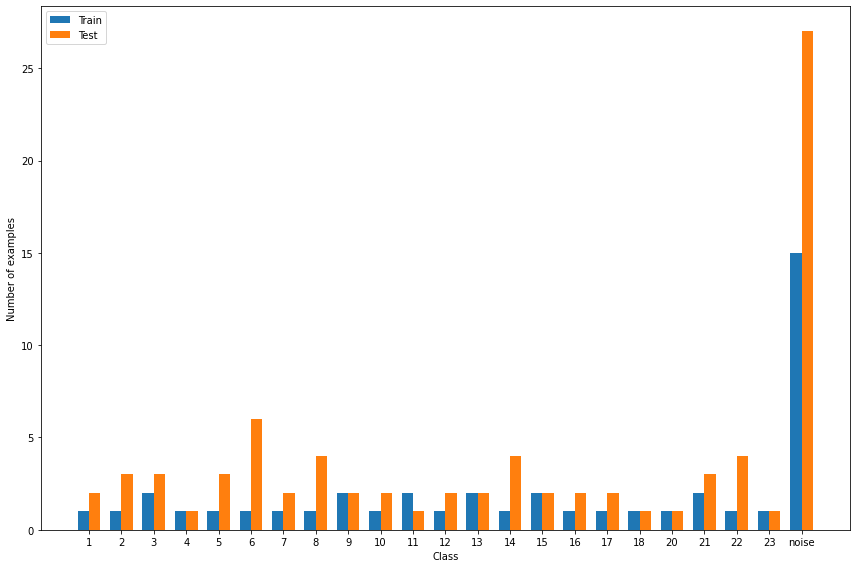
\includegraphics[scale=0.38]{Chapter6/figs/SDRP-class-dist.png}
	\end{center}
	\caption{The class distribution for the SDRP dataset, split by set.}
	\label{fig:sdrp-dist}
\end{figure}

These properties lead to the SDRP dataset being extremely challenging for an SNN to train on. However it is also an accurate representation of what a real life photo-id catalogue dataset would look like in the initial stages of a survey, providing an excellent test of both the robustness and generalisability of the SNN-based approach to automatic most likely catalogue matching when only small amounts of training data are available. 

\section{Siamese Neural Network Evaluation Using the SDRP Dataset}\label{ch:SNNGeneralisation,sec:SNNEvalWithSDRP}




